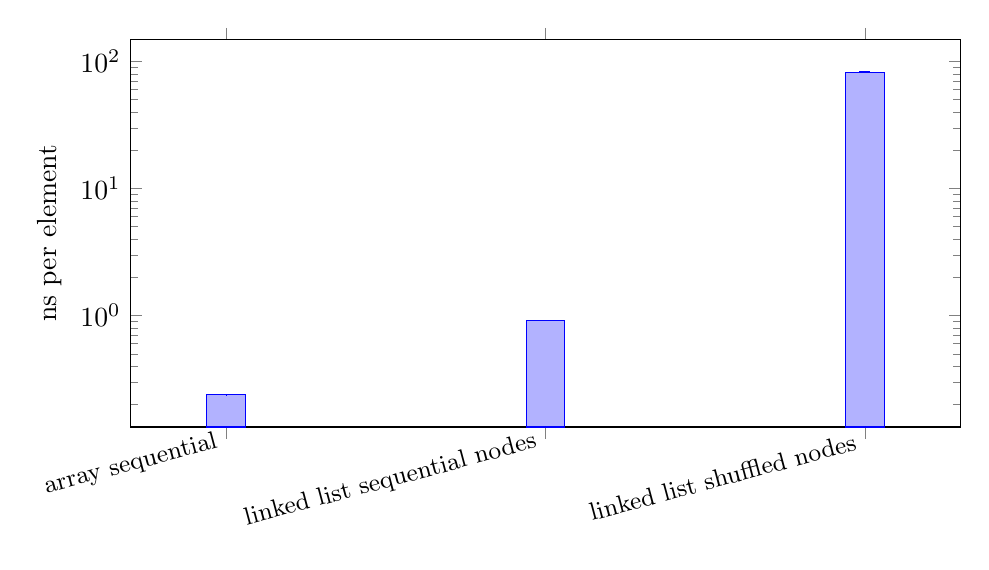
\begin{tikzpicture}
\begin{axis}[ybar, width=\textwidth, height=6.5cm, bar width=14pt, ymode=log, log origin=infty, symbolic x coords={array sequential,linked list sequential nodes,linked list shuffled nodes}, xtick=data, x tick label style={rotate=15, anchor=east, font=\small}, ylabel={ns per element}, enlarge x limits=0.15, legend style={font=\small, at={(0.98,0.98)}, anchor=north east}, nodes near coords, nodes near coords style={font=\tiny}, every node near coord/.append style={/pgf/number format/.cd, fixed, precision=2}, nodes near coords={}]
\addplot+[error bars/.cd, y dir=both, y explicit] coordinates {(array sequential,0.2390) +- (0,0.0010) (linked list sequential nodes,0.9176) +- (0,0.0042) (linked list shuffled nodes,82.2320) +- (0,0.4010)};
\end{axis}
\end{tikzpicture}